\documentclass[a4paper,12pt]{article} 
\usepackage[francais]{babel}
\usepackage[T1]{fontenc} 
\usepackage[utf8]{inputenc} 
\usepackage{graphicx}
\usepackage{color}
\usepackage{hyperref}
\usepackage{fontspec}
\begin {document}
\begin {figure}

\includegraphics[width=0.3\textwidth]{logolemansU.png}
\hspace{150pt} 

\includegraphics[width=0.3\textwidth] {logo_ic2.png}
\end {figure}
\title {\textbf {\color {blue} Le Mans Université}\color{black}
\\  Licence Informatique  \textit {2ème année}
 \\Module Projet
 \\\\\\ \textbf {Bataille navale en réseau}}
\author{DEROUET Corentin & GERARD Jules & DEUX Killian}
% \author{\href{mailto: prenom.nom.etu@univ-lemans.fr} {prenom.nom.etu@univ-lemans.fr}}

\date{\today} 
\maketitle \newpage
\newpage
\tableofcontents
\newpage


 
\section {Introduction}
 	Dans le cadre de l'unité d'enseignement « conduite de projet », il nous a été demandé de coder un jeu en langage C à plusieurs. \vspace{2\baselineskip}\\
    L'objectif de ce projet est de mettre à contribution des enseignements appris depuis notre début de cursus tel que « Algorithmique ». Cela permettra de nous former au travail à plusieurs, une grande nouveauté pour nous. Le but est donc de coder un jeu en respectant un cahier des charges défini en amont.\\
    Nous avons alors décidé le sujet d’une « bataille navale ». C'est un jeu de société qui, dans sa forme originale, se joue à deux joueurs dans lequel chacun d'entre eux doivent placer des bateaux sur une grille, inconnue de l'adversaire, et tenter de trouver les bateaux ennemis. La partie se termine lorsque l'un des joueurs arrive à trouver tous les bateaux de son adversaire avant que tous les siens ne soient découvert. Chaque joueur dispose alors de deux grilles. La première grille servira à placer ses bateaux et la seconde à placer des pions. Cette seconde grille sera une vue de la grille adverse. Lors d'un tir à des coordonnées précise dans la grille adverse, l'ennemi nous indiquera si notre tir a atterri « dans l'eau » , a « touché » un bateau ou a « coulé » un bateau. C'est en fonction de ces informations que l'on peut placer sur notre seconde grille un pion de différente couleur. Nous avons cependant changé quelques règles que nous avons défini en début de projet. \\
 
\newpage
\section {Organisation}
La planification du projet a été articulée autour de l'outil "Projects" de GitHub.\\
Celui-ci permet, via un système de "cartes", d'assigner des tâches à chacun d'entre nous.\\
\begin{center}
  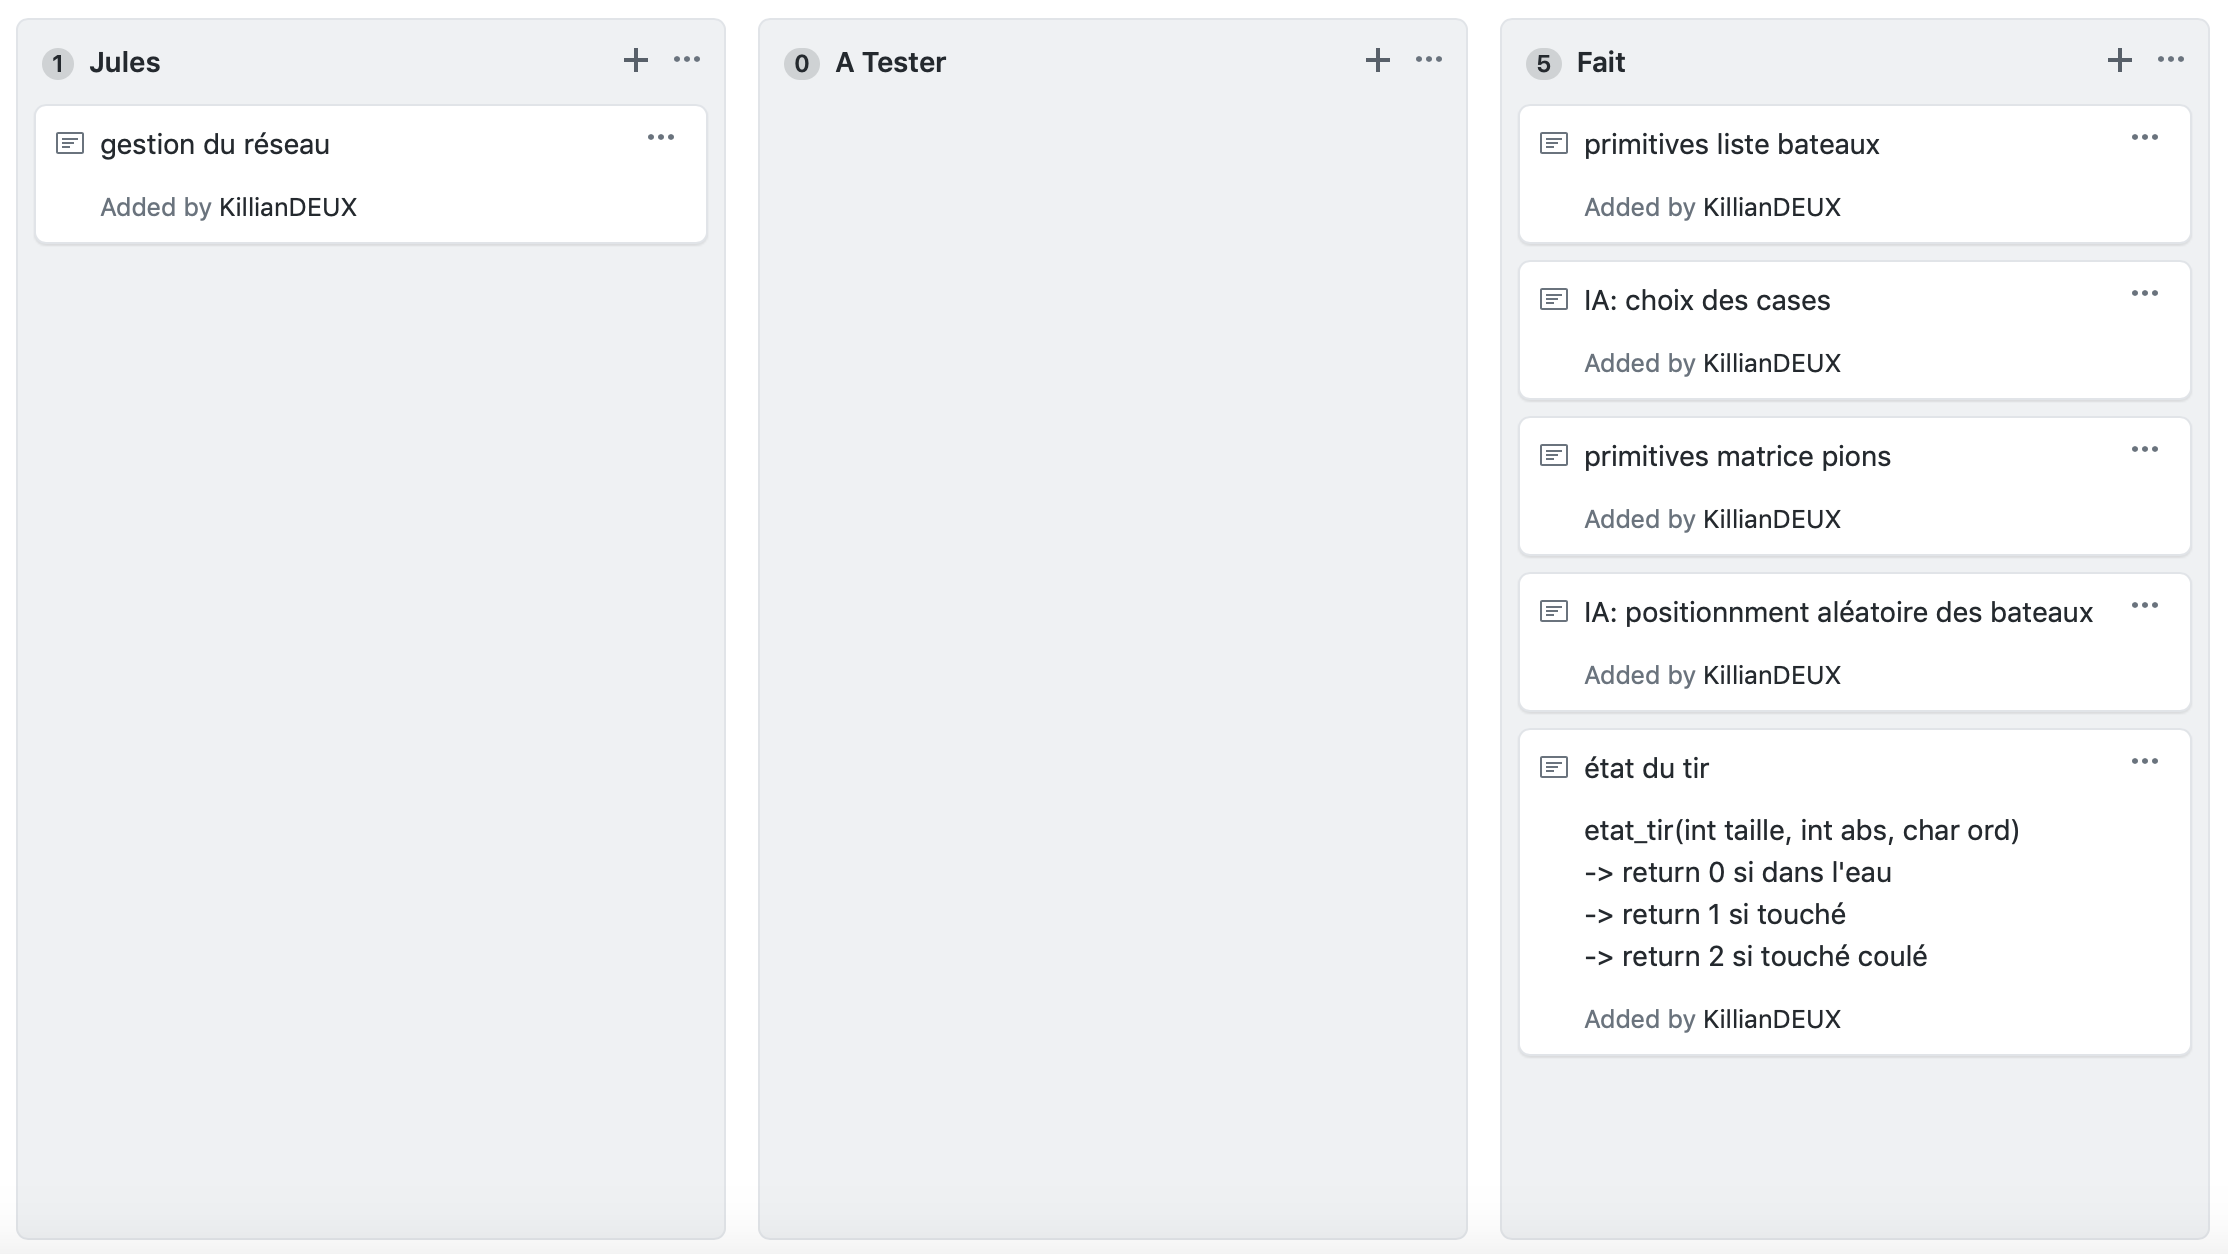
\includegraphics[width=1\textwidth] {capture_projects.png}  
  Figure 1 - Planificateur GitHub 
\end{center}
Ainsi que autour de l'outil "Code"  également de GitHub.\\
Cet outil permet de récupérer et de mettre à jour les changements effectués dans le code.\\
\\
La répartition globale est la suivante : \\
- Killian : gestion des bateaux et des opérations sur les matrices \\
- Corentin : gestion des matrices de pions et du mode jeu IA \\
- Jules : protocole de communication et gestion du réseau \\



\newpage
\section {Conception/Analyse}
\subsection {Présentation approfondie}
blabla
\newpage
\subsection {Explication des règles}
blabla
\subsection {Explication des fonctionnalités}

\newpage
\section {Développement}
\subsection {Présentation de la conception d'un bateau}
blabla
\newpage
\subsection {Présentation de la matrice et des pions}
blabla
\newpage
\subsection {Présentation de l'IA}
blabla
\newpage
\subsection {Présentation du réseau}
Pour permettre l’échange de données entre les différents utilisateurs, nous avons choisi d’implanter le réseau dans ce projet grâce au protocole TCP. Celui-ci présente comme un avantage important : le contrôle de l’information reçue.
\\ Comme le jeu doit supporter un nombre variable de joueur, le serveur est en mesure d’ouvrir plusieurs sockets clients.
\\ Pour cela, il a été nécessaire de faire un tableau pour établir les canaux de communication de chaque client. Ainsi, le canal d’indice 0, correspond au 1er client qui s’est connecté et ainsi de suite.
\\image socket client.
\\ Ces canaux vont permettre d’envoyer des variables par le réseau via les fonctions send et recv de la bibliothèque « ... ».
\\ Ce mode de fonctionnement est adapté au jeu de la bataille navale tour par tour car la fonction recv est bloquante. 
\\ La main est rendu à l’utilisateur dès que l’information est reçue, dans le cas contraire, celui-ci reste en attente.

\newpage

\newpage
\section {Résultat} 
blabla

\newpage
\section {Conclusion} 
blabla

\newpage
\section {Annexe}  blabla

\begin{thebibliography} {99}
\bibitem[1]{x1} \url http://benhur.teluq.uquebec.ca/~mcouture/apa/index.htm
\bibitem[2]{x2} \url http://benhur.teluq.uquebec.ca/~mcouture/apa/docsweb.htm
\end {thebibliography}
\end {document}